\documentclass{ctexart}

\usepackage{setspace}
\usepackage{booktabs}
\usepackage{amsmath}
\usepackage{amsfonts}
\usepackage{amsthm}
\usepackage{amssymb} 

\usepackage{graphicx}

\title{概率论笔记}
\author{杨子颉}

\begin{document}
\maketitle
\newpage
\tableofcontents
\newpage
\section{随机事件及其概率}
    \subsection{样本空间与随机事件}
        随机试验具有以下的特点：可重复性、所有结果可确定性、每次结果不确定性

        样本空间：随机试验的所有可能结果组合的集合（基本事件组）

        随机事件：随机试验的样本空间的子集称为随机事件。

        基本事件：样本点组成的单点集；最小的随机事件，无法再往下分解，

        \subsection{事件间的关系与运算}
        事件间的关系与运算应按照集合间的关系与运算来规定

        包含关系：$A\subset B$事件A是B的子事件，即A发生B必然发生（小推大）

        互斥事件：事件A和事件B不能同时发生即$A\cap B= \varnothing$ 
        \begin{figure}[h]
            \centering
            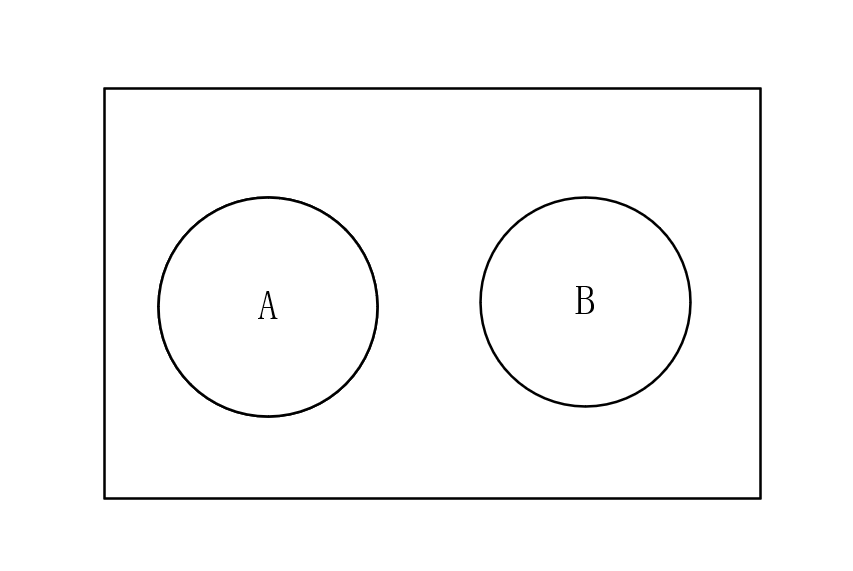
\includegraphics[width=0.4\textwidth]{Figure/互斥.png}
            \caption{互斥事件}
        \end{figure}


        对立事件：事件A不可能发生的事件，记作$\bar{A}$
        \begin{figure}[h]
            \centering
            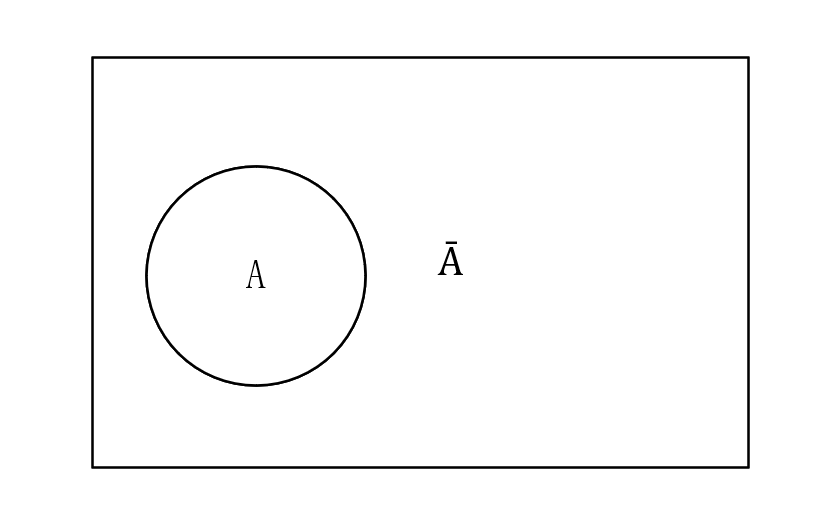
\includegraphics[width=0.4\textwidth]{Figure/QQ20260306-145147.png}
            \caption{对立事件}
        \end{figure}

        和事件：事件A和事件B至少有一个发生，记作$A \cup B$

        差事件：事件A发生而B不发生，记作$A-B$，特别的，$\Omega -B$记作$\bar{B}$

        积事件：事件A和事件B同时发生，记为$A \cap B$




\end{document}